%\documentclass[landscape,a0b,final,a4resizeable]{a0poster}
%\documentclass[landscape,a0b,final]{a0poster}
%\documentclass[portrait,a0b,final,a4resizeable]{a0poster}
\documentclass[portrait,a0b,final]{a0poster}
%%% Option "a4resizeable" makes it possible ot resize the
%   poster by the command: psresize -pa4 poster.ps poster-a4.ps
%   For final printing, please remove option "a4resizeable" !!

\usepackage{epsfig}
\usepackage{multicol}
\usepackage{pstricks,pst-grad}
\usepackage{graphicx}% Include figure files
\usepackage{dcolumn}% Align table columns on decimal point
\usepackage{bm}% bold math
\usepackage{epsf}
\usepackage{enumitem}
\usepackage{pifont}
\usepackage{amsmath,amssymb,amsfonts}
\usepackage{xcolor}
\usepackage{tikz}
\usepackage{mathtools}


\newcommand{\bra}[1]{\left\langle #1\right|}
\newcommand{\ket}[1]{\left|#1\right\rangle}
\newcommand{\braket}[2]{\left\langle #1|#2\right\rangle}
\newcommand{\ketbrad}[1]{|#1\rangle\!\langle #1|}
\newcommand{\tr}[1]{\mathrm{tr}\left\{#1\right\}}
\newcommand{\ptr}[2]{\mathrm{tr_{#1}}\left\{#2\right\}}
\newcommand{\di}[1]{\mathrm{div}\left\{#1\right\}}
\newcommand{\la}{\left\langle}
\newcommand{\ra}{\right\rangle}
\newcommand{\pd}{\partial}
\newcommand{\de}[1]{\delta\left[#1\right]}
\newcommand{\td}{\mathrm{d}}
\newcommand{\ma}[1]{\max{\left\{#1\right\}}}
\newcommand{\mi}[1]{\min{\left\{#1\right\}}}
\newcommand{\etal}{\textit{et al. }}
\newcommand{\e}[1]{\exp{\left(#1\right)}}
\newcommand{\lo}[1]{\ln{\left(#1\right)}}
\newcommand{\id}{\mathbb{I}}
\newcommand{\com}[2]{\left[#1,\,#2\right]}
\newcommand{\acom}[2]{\left\{#1,\,#2\right\}}
\newcommand{\co}[1]{\cos{\left(#1\right)}}
\newcommand{\si}[1]{\sin{\left(#1\right)}}
\newcommand{\sh}[1]{\sinh{\left(#1\right)}}
\newcommand{\ch}[1]{\cosh{\left(#1\right)}}
\newcommand{\shi}[1]{\mathrm{shi}{\left(#1\right)}}
\newcommand{\cohi}[1]{\mathrm{chi}{\left(#1\right)}}
\newcommand{\ct}[1]{\coth{\left(#1\right)}}
\newcommand{\bla}{bla\\bla\\bla\\bla\\bla}
%\newcommand{\eqref}[1]{(\ref{#1})}
\newcommand{\PR}{Phys. Rev.}
\newcommand{\PRA}{Phys. Rev. A }
\newcommand{\PRB}{Phys. Rev. B }
\newcommand{\PRD}{Phys. Rev. D }
\newcommand{\PRE}{Phys. Rev. E }
\newcommand{\PRL}{Phys. Rev. Lett. }
\newcommand{\PRX}{Phys. Rev. X }
\newcommand{\EPL}{EPL (Europhys. Lett.) }
\newcommand{\RMP}{Rev. Mod. Phys. }
\newcommand{\NJP}{New. J. Phys. }




\newcommand{\mb}[1]{\mbox{\boldmath$#1$}}
\newcommand{\mc}[1]{\mathcal{#1}}
\newcommand{\mbb}[1]{\mathbb{#1}}
\newcommand{\mf}[1]{\mathfrak{#1}}
\newcommand{\mrm}[1]{\mathrm{#1}}
\newcommand{\clr}{\color{red}}



\newcommand{\ptl}[3]{\left( \frac{\partial {#1}}{\partial {#2}} \right)_{#3}}

\def\dbar{{\mathchar'26\mkern-12mu {\rm d}}}

\DeclareMathOperator*{\sumint}{%
\mathchoice%
  {\ooalign{$\displaystyle\sum$\cr\hidewidth$\displaystyle\int$\hidewidth\cr}}
  {\ooalign{\raisebox{.14\height}{\scalebox{.7}{$\textstyle\sum$}}\cr\hidewidth$\textstyle\int$\hidewidth\cr}}
  {\ooalign{\raisebox{.2\height}{\scalebox{.6}{$\scriptstyle\sum$}}\cr$\scriptstyle\int$\cr}}
  {\ooalign{\raisebox{.2\height}{\scalebox{.6}{$\scriptstyle\sum$}}\cr$\scriptstyle\int$\cr}}
}

\newcommand{\bull}{\ding{217}}
\newcommand{\ite}{\vspace{0.1em}\item\hspace{1em}}


%%%%%%%%%%%%%%%%%%%%%%%%%%%%%%%%%%%%%%%%%%%
% Definition of some variables and colors
%\renewcommand{\rho}{\varrho}
%\renewcommand{\phi}{\varphi}
\setlength{\columnsep}{3cm}
\setlength{\columnseprule}{1mm}
\setlength{\parindent}{0.0cm}



%%%%%%%%%%%%%%%%%%%%%%%%%%%%%%%%%%%%%%%%%%%%%%%%%%%%
%%%               Background                     %%%
%%%%%%%%%%%%%%%%%%%%%%%%%%%%%%%%%%%%%%%%%%%%%%%%%%%%
\newcommand{\background}[3]{
  \newrgbcolor{cgradbegin}{#1}
  \newrgbcolor{cgradend}{#2}
  \psframe[fillstyle=gradient,gradend=cgradend,
  gradbegin=cgradbegin,gradmidpoint=#3](0.,0.)(1.\textwidth,-1.\textheight)
}





%%%%%%%%%%%%%%%%%%%%%%%%%%%%%%%%%%%%%%%%%%%%%%%%%%%%
%%%                Poster                        %%%
%%%%%%%%%%%%%%%%%%%%%%%%%%%%%%%%%%%%%%%%%%%%%%%%%%%%

\newenvironment{poster}{
  \begin{center}
  \begin{minipage}[c]{0.98\textwidth}
}{
  \end{minipage} 
  \end{center}
}



%%%%%%%%%%%%%%%%%%%%%%%%%%%%%%%%%%%%%%%%%%%%%%%%%%%%
%%%                pcolumn                       %%%
%%%%%%%%%%%%%%%%%%%%%%%%%%%%%%%%%%%%%%%%%%%%%%%%%%%%

\newenvironment{pcolumn}[1]{
  \begin{minipage}{#1\textwidth}
  \begin{center}
}{
  \end{center}
  \end{minipage}
}



%%%%%%%%%%%%%%%%%%%%%%%%%%%%%%%%%%%%%%%%%%%%%%%%%%%%
%%%                pbox                          %%%
%%%%%%%%%%%%%%%%%%%%%%%%%%%%%%%%%%%%%%%%%%%%%%%%%%%%

\newrgbcolor{lcolor}{0. 0. 0.80}
\newrgbcolor{gcolor1}{1. 1. 1.}
\newrgbcolor{gcolor2}{.80 .80 1.}

\newcommand{\pbox}[4]{
\psshadowbox[#3]{
\begin{minipage}[t][#2][t]{#1}
#4
\end{minipage}
}}











%%%%%%%%%%%%%%%%%%%%%%%%%%%%%%%%%%%%%%%%%%%%%%%%%%%%%%%%%%%%%%%%%%%%%%
%%% Begin of Document
%%%%%%%%%%%%%%%%%%%%%%%%%%%%%%%%%%%%%%%%%%%%%%%%%%%%%%%%%%%%%%%%%%%%%%

\begin{document}

\background{0 0 0}{.99 .71 .08}{0.2}


\vspace*{1cm}


\newrgbcolor{line}{0 0 0}
\newrgbcolor{white}{.995, .995, .995}
\newrgbcolor{gray}{.97, .97, .97}
\definecolor{UMBC black}{RGB}{0 0 0}
\definecolor{UMBC gold}{RGB}{253 181 21}



\begin{poster}

%%%%%%%%%%%%%%%%%%%%%
%%% Header
%%%%%%%%%%%%%%%%%%%%%
\begin{center}
\begin{pcolumn}{0.98}

\pbox{0.97\textwidth}{0.09\textheight}{linewidth=2mm,framearc=0.3,linecolor=line,fillstyle=gradient,gradangle=0,gradbegin=white,gradend=gray,gradmidpoint=1.0,framesep=1em}{
\vspace{0.5em}
%%% Unisiegel
\begin{minipage}[c][7.5cm][c]{0.1\textwidth}
  \begin{center}
    
\includegraphics[height=7.5cm,angle=0]{UMBC-logo_small.eps}
  \end{center}
\end{minipage}
%%% Titel
\begin{minipage}[c][10cm][c]{0.78\textwidth}
  \begin{center}
    {\sc \huge Simon's algorithm in the NISQ cloud}\\[9mm]
    {\Large Reece Robertson, Emery Doucet, Ernest Spicer, and Sebastian Deffner\\[6mm]
    Department of Physics, University of Maryland Baltimore County, Baltimore, Maryland 21250, USA \\[1mm]
    }
  \end{center}
\end{minipage}
%%% GK-Logo
\begin{minipage}[c][7.5cm][c]{0.1\textwidth}
  \begin{center}
    
\includegraphics[height=7.5cm,angle=0]{UMBC-logo_small.eps}
  \end{center}
\end{minipage}

}
\end{pcolumn}
\end{center}


\vspace*{1cm}



%%%%%%%%%%%%%%%%%%%%%
%%% Content
%%%%%%%%%%%%%%%%%%%%%
\begin{center}
 


\begin{pcolumn}{0.495}
\pbox{0.9\textwidth}{0.09\textheight}{linewidth=2mm,framearc=0.1,linecolor=line,fillstyle=gradient,gradangle=0,gradbegin=white,gradend=white,gradmidpoint=1.0,framesep=1em}{
\vspace{1cm}\begin{center}\pbox{0.8\textwidth}{}{linewidth=2mm,framearc=0.3,linecolor=line,fillstyle=gradient,gradangle=0,gradbegin=white,gradend=gray,gradmidpoint=1.0,framesep=1em}{\begin{center}\textbf{Abstract}\end{center}}\end{center}
\vspace{1.25cm}

Simon's algorithm demonstrates genuine quantum advantage, however, it assumes access to noise-free qubits.
We use Simon's algorithm to benchmark the error rates of devices currently available in the ``quantum cloud.''
Our main result is a comparison between the platforms made available by IBM and IonQ.
This highlights the importance of understanding device architectures when transpiling quantum algorithms onto hardware.
For instance, we show that two-qubit operations between distant superconducting qubits should be avoided.

}

\vspace*{0.01\textheight}

\pbox{0.9\textwidth}{0.23\textheight}{linewidth=2mm,framearc=0.1,linecolor=line,fillstyle=gradient,gradangle=0,gradbegin=white,gradend=white,gradmidpoint=1.0,framesep=1em}{
\vspace{1cm}\begin{center}\pbox{0.8\textwidth}{}{linewidth=2mm,framearc=0.3,linecolor=line,fillstyle=gradient,gradangle=0,gradbegin=white,gradend=gray,gradmidpoint=1.0,framesep=1em}{\begin{center}\textbf{Background}\end{center}}\end{center}\vspace{1.25cm}

Simon's problem takes as input an oracle function $U_f$ which operates on bitstrings of size $n$.
The function is either one-to-one, or two-to-one with a fixed secret string $s$ that relates each pair of inputs.
The objective is to classify the provided function into one of the two classes.
Simon invented a quantum algorithm which completes this task in polynomial time, while a classical computer must run a probabilistic calculation with an exponential expected runtime.~\cite{ref1}

\begin{center}
  
\includegraphics[height=4.5cm,angle=0]{genericAlgorithm.png}
\end{center}

Above is the quantum circuit diagram for Simon's algorithm.
Note the use of two quantum registers of size $n$, both initialized to the state $|0\rangle$, as well as the oracle $U_f$.
The algorithm uses two Hadamard transformations and $U_f$ to create a superposition over all the size $n$ bitstrings that are orthogonal to the secret string $s$.
An iteration of the algorithm is successful if the final measurement result is indeed orthogonal to $s$ (this is always true in the noise free case).
The entire algorithm is successful if a complete set of $n-1$ linearly independent bitstrings are measured and the resulting system is solved classically in polynomial-time.

}

\vspace*{0.01\textheight}

\pbox{0.9\textwidth}{0.45\textheight}{linewidth=2mm,framearc=0.1,linecolor=line,fillstyle=gradient,gradangle=0,gradbegin=white,gradend=white,gradmidpoint=1.0,framesep=1em}{
\vspace{1cm}\begin{center}\pbox{0.8\textwidth}{}{linewidth=2mm,framearc=0.3,linecolor=line,fillstyle=gradient,gradangle=0,gradbegin=white,gradend=gray,gradmidpoint=1.0,framesep=1em}{\begin{center}\textbf{The Quantum Cloud}\end{center}}\end{center}\vspace{1.25cm}

Several large corporations as well as smaller start-up companies have made their NISQ devices available for cloud access.
This offers exciting prospects for fundamental as well as applied research, as now with comparatively little effort ``quantum experiments'' can be performed.
However, it has also already been demonstrated that the reported \emph{quantum volume}\footnote{The \emph{quantum volume} is defined using the number of qubits and the number of operations that can be effectively implemented on the device.}
often overestimates what is experimentally accessible.

This raises the somewhat natural question, how do algorithms designed for the very purpose of exhibiting quantum advantage perform on available NISQ devices?
For our study, we had access to IBM's superconducting platform and IonQ's trapped ion devices.

\textbf{Superconducting qubits -- IBM:}
Quantum processors are made up superconducting transmon qubits are located in dilution refrigerators at the IBM Research headquarters at the Thomas J. Watson Research Center.
For our work, we used the 127-qubit Brisbane, Osaka, and Kyoto superconducting quantum processors, for which noisy simulators are also provided.
The device topologies for each quantum processing unit are depicted below (note that all are instances of the IBM Eagle chip design).


\begin{center}
  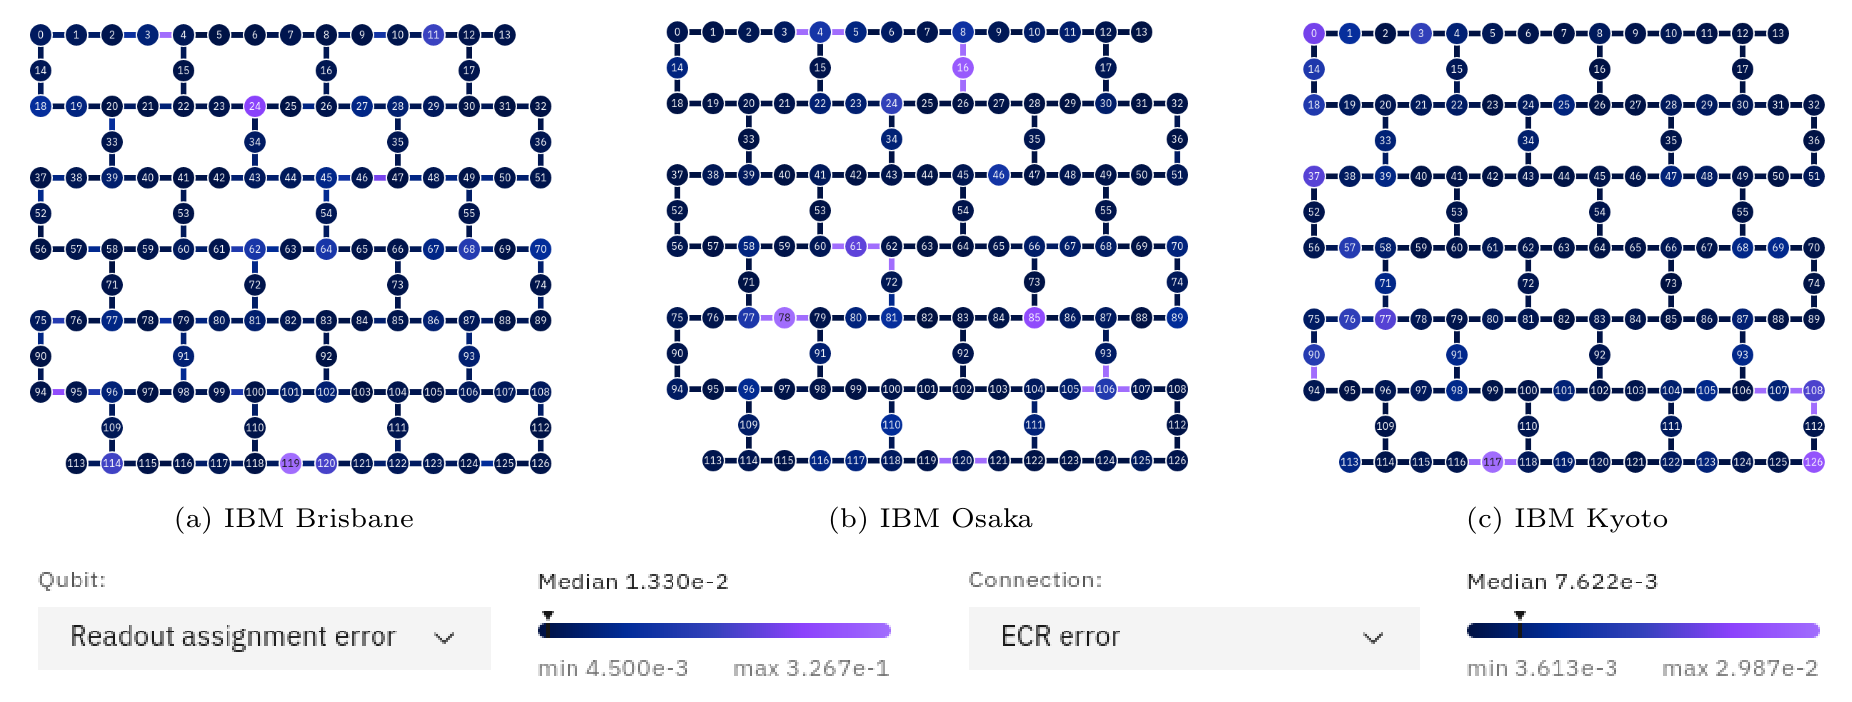
\includegraphics[height=12cm,angle=0]{ibmDevices.png}
\end{center}

\textbf{Ion traps -- IonQ:}
A fundamentally different type of system are the trapped ion devices of IonQ, which are physically located here in College Park, Maryland.
Typically, trapped ion NISQ devices exhibit several advantages, such as accuracy, predictability, and coherence time.
However, such systems have the disadvantage that the number of qubits is much smaller.
For instance, the largest IonQ device (Forte) has only 36 qubits.
Some of the limitations arising from the small qubit number is made up by the fact that trapped ion computers possess full connectivity.

\begin{center}
  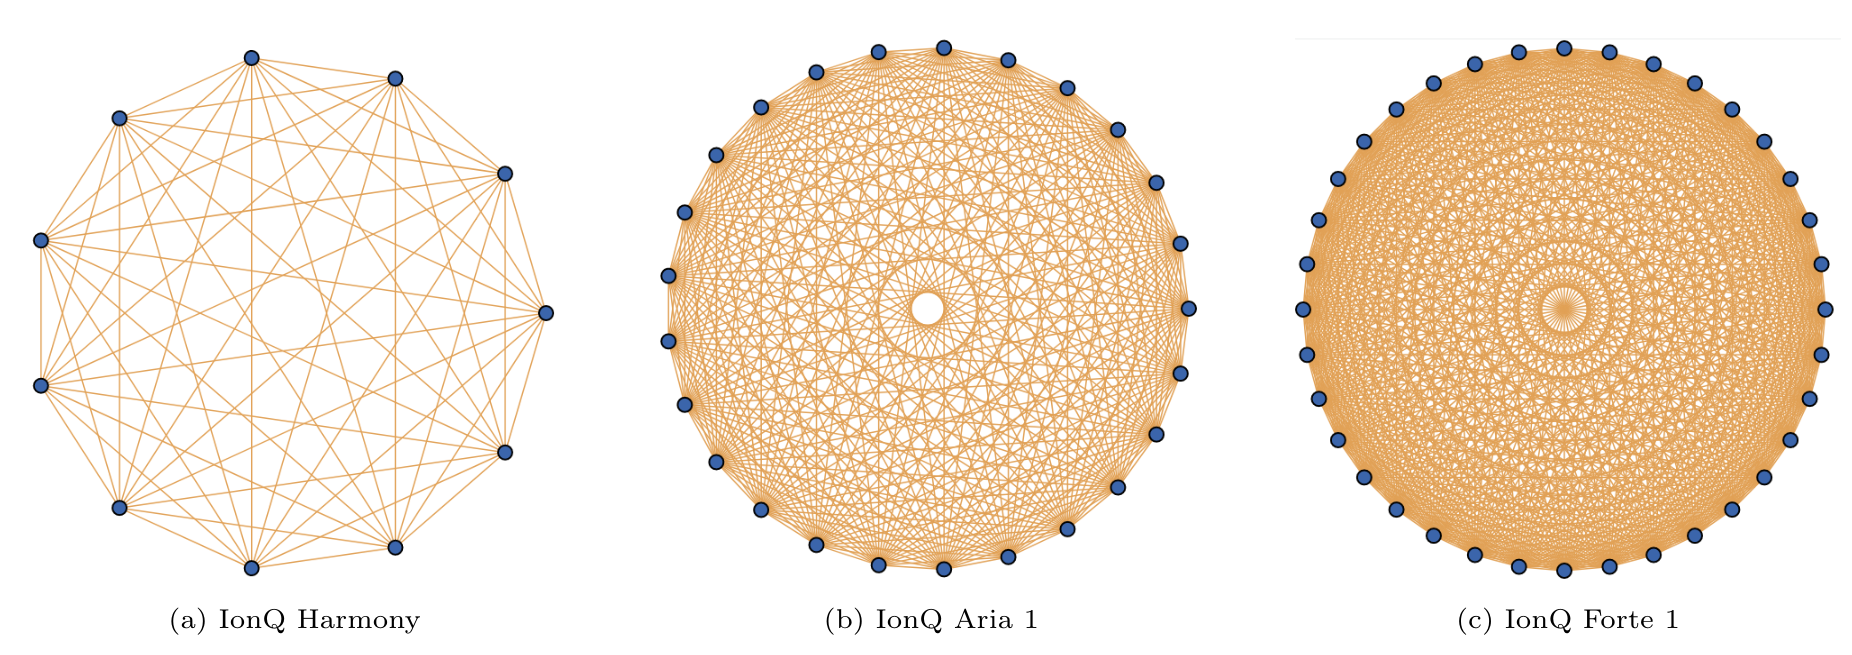
\includegraphics[height=12cm,angle=0]{ionqDevices.png}
\end{center}

}

\end{pcolumn}
\begin{pcolumn}{0.495}
\pbox{0.9\textwidth}{0.54\textheight}{linewidth=2mm,framearc=0.1,linecolor=line,fillstyle=gradient,gradangle=0,gradbegin=white,gradend=white,gradmidpoint=1.0,framesep=1em}{

\vspace{1cm}\begin{center}\pbox{0.8\textwidth}{}{linewidth=2mm,framearc=0.3,linecolor=line,fillstyle=gradient,gradangle=0,gradbegin=white,gradend=gray,gradmidpoint=1.0,framesep=1em}{\begin{center}\textbf{Methods \& Results}\end{center}}\end{center}\vspace{1.25cm}

We ran Simon's algorithm on the IBM superconducting and IonQ trapped ion quantum devices listed in ``The Quantum Cloud'' section.
We also ran Simon's algorithm on each devices' corresponding simulator.
Our process was as follows:
\begin{enumerate}
  \item We initialized a variable $n$ to iterate over the values 2—12.
  \item For each $n$, we defined a two-to-one function using the string of $n$ 1s as the secret string $s$.
  This represents the most complex oracle in terms of the number of two-qubit gates required to implement it.
  \item We prepared an implementation of Simon's algorithm to classify this function.
  \item We repeated the implementation 8192 times.
  \item We counted the number of times the implementation produced a final result which was not orthogonal to $s$, indicating a failure of the algorithm (the ``algorithmic error'').
  \item We averaged the algorithmic error of each device over many repetitions of steps 1-5, and plotted the results.
\end{enumerate}
Our findings are presented in the figures below.
The first plot shows the algorithmic error on each IonQ device and simulator scales linearly.
This indicates two things: first, that the IonQ devices scale consistently throughout the ``intermediate scale,'' and second, IonQ simulators agree with the general behavior of the real devices (up to a constant factor).
However, with an observed 30\% algorithmic error for $n=12$, the IonQ devices are not performing particularly well---we expect this amount of error to nullify quantum advantage.

\begin{center}
  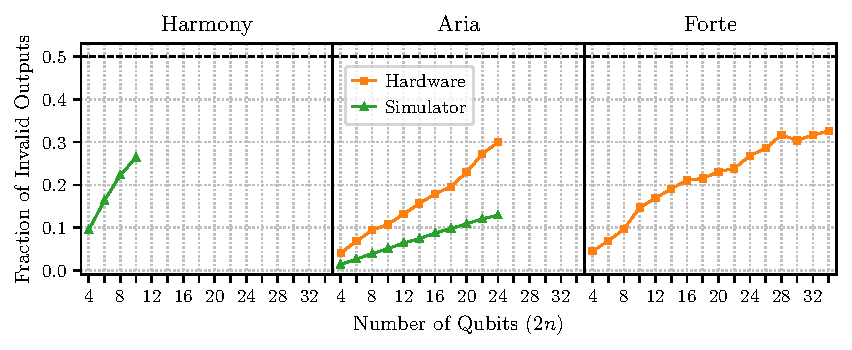
\includegraphics[height=12cm,angle=0]{IonQComparisonTest.pdf}
\end{center}

The second plot shows that IBM Brisbane experiences a nonlinear jump in algorithmic error at $n=4$, and by the moderately sized $n>8$, the algorithm fails entirely for this oracle.
More curious is the output of the noisy simulators.
The IBM AER local simulators all predict a roughly linear scaling in algorithmic error as problem size increases, similar to what was observed on IonQ but in sharp contrast to the IBM results.

A plausible hypothesis is that this increase in error on superconducting hardware coincides with the addition of a number of swap gates into the algorithm due to the limited chip layout.
Interestingly, however, the simulated algorithm also has swap gates of the same pattern, but the jump in error is not observed.
Thus, the dramatic jump in algorithmic error observed on the hardware may be due to correlated errors that accompany the addition of the swap operations which is not captured in the noise model of the simulators. 

\begin{center}
  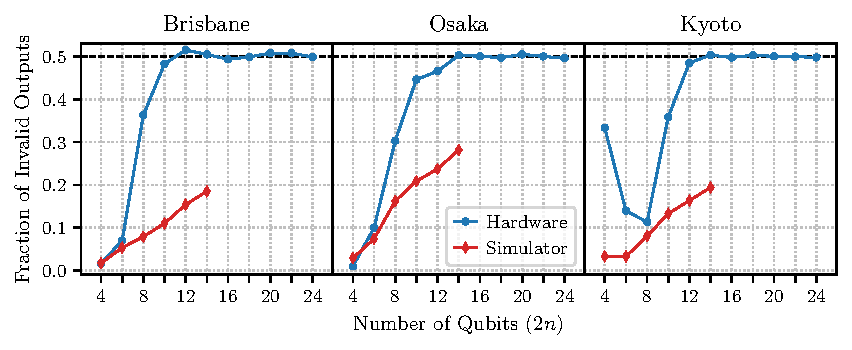
\includegraphics[height=12cm,angle=0]{IBMComparisonTest.pdf}
\end{center}

In short, we find that the algorithmic error of Simon's algorithm on NISQ devices scales at least linearly, and all devices show irrecoverable error for intermediate-scale problems ($n=12$).

}

\vspace*{0.01\textheight}


\pbox{0.9\textwidth}{0.20\textheight}{linewidth=2mm,framearc=0.1,linecolor=line,fillstyle=gradient,gradangle=0,gradbegin=white,gradend=white,gradmidpoint=1.0,framesep=1em}{

\vspace{1cm}\begin{center}\pbox{0.8\textwidth}{}{linewidth=2mm,framearc=0.3,linecolor=line,fillstyle=gradient,gradangle=0,gradbegin=white,gradend=gray,gradmidpoint=1.0,framesep=1em}{\begin{center}\textbf{Physical Parameters of the NISQ Devices}\end{center}}\end{center}\vspace{1.25cm}

\begin{center}
  \begin{tabular}{|c|c|c|c|c|c|c|}
    \hline
    Parameter & Brisbane & Osaka & Kyoto & Forte & Aria 1 & Harmony \\
    \hline
    \hline
    Manufacturer & IBM & IBM & IBM & IonQ & IonQ & IonQ \\
    \hline
    T1 Time & 213.12 $\mu$s & 297.17 $\mu$s & 215.43 $\mu$s & 100 s & 100 s & 10000 s \\
    \hline
    T2 Time & 145.97 $\mu$s & 127.23 $\mu$s & 109.44 $\mu$s & 1 s & 1 s & 0.2 s \\
    \hline
    2-Qubit Gate Speed & 660 ns & 660 ns & 660 ns & 970 $\mu$s & 600 $\mu$s & 200 $\mu$s \\
    \hline
    1-Qubit Gate Error (\%) & 0.03 & 0.03 & 0.03 & 0.09 & 0.06 & 0.67 \\
    \hline
    2-Qubit Gate Error (\%) & 0.74 & 0.93 & 0.92 & 0.74 & 8.57 & 3.07 \\
    \hline
    Average Readout Error (\%) & 1.32 & 2.18 & 1.48 & 0.5 & 0.52 & 0.42 \\
    \hline
    Topology & Eagle r3 & Eagle r3 & Eagle r3 & all-to-all & all-to-all & all-to-all \\
    \hline
  \end{tabular}
\end{center}

Performance metrics for IBM and IonQ devices.
Note that for one and two qubit gate errors and times, IBM reports median values while IonQ reports average values.
The native gate set supported by the IBM devices includes: ECR, ID, RZ, SX, and X gates; while the native gate set for the IonQ devices consists of: MS, GPI, and GPI2 gates (IonQ Forte also implements ZZ gates natively).

}

\vspace*{0.01\textheight}

\pbox{0.9\textwidth}{0.03\textheight}{linewidth=2mm,framearc=0.1,linecolor=line,fillstyle=gradient,gradangle=0,gradbegin=white,gradend=white,gradmidpoint=1.0,framesep=1em}{


%%% References
\begin{thebibliography}{80}

\bibitem{ref1} D. R. Simon, On the power of quantum computation, SIAM Journal on Computing 26 (5) (1997) 1474--1483. arXiv:
https://doi.org/10.1137/S0097539796298637, doi:10.1137/S0097539796298637.

\end{thebibliography}
}

\end{pcolumn}

\end{center}

\end{poster}

\end{document}

\bib